\chapter{Experimentos}
\label{cap:experimentos}

Como se ha comentado en el apartado del \ref{cap:estadoDeLaCuestion}, la investigación acerca de este tema sigue en curso y todavía no hay una solución generalista para reemplazar los solvers físicos con modelos de Machine Learning. Utilizando la infraestructura descrita en el capítulo anterior, se ha comparado la efectividad de modelos con diferentes características, con el fin de analizar las limitaciones de esta alternativa y descubrir qué técnicas resultan ser más prometedoras. \newline

A la hora de valorar la calidad de un sistema de inferencia en tiempo de ejecución, hay dos criterios fundamentales:
\begin{itemize}
  \item \textit{Rendimiento}: Los modelos deben ser capaces de competir con los reducidos tiempos de cómputo de los solvers. Para ello, tanto los modelos como los datos de input han de ser lo más ligeros posibles. Las métricas que se emplean para medir la calidad del rendimiento son las siguentes: 
  \begin{itemize}
    \item \textit{Tiempo de entrenamiento}: medido en minutos/horas (m, h), el tiempo necesario transcurrido para entrenar un modelo a partir de un dataset. Incluye tanto el entrenamiento como el testing que proporciona las métricas. 
    \item \textit{Tiempo de inferencia}: medido en milisegundos (ms), es el tiempo medio de inferencia de un modelo en ejecución en el entorno de simulación. Abarca desde que se pide una respuesta al modelo hasta que se obtienen los datos. \footnote{No se ven reflejados los procesos adicionales que se llevan a cabo en Unity como podría ser el cálculo del PCA para un frame.}
    \item \textit{Error medio por vértice}: medido en metros (m), es el error medio de predicción de un batch, es decir la diferencia media que se encuentra entre las posiciones predichas y reales de los vértices. Se calcula en la fase de prueba del entrenamiento para cada primer frame de un batch \footnote{Para calcular el error de vértice del primer frame de un batch, se compara el último predicho de \textit{batch\_seq} con el primero de \textit{batch\_future}.}.
    \item \textit{Frames por segundo}: (FPS) la media calculada durante la simulación. 
  \end{itemize}
    Las métricas que se calculan durante la simulación en Unity, el tiempo de inferencia y las FPS, se medirán en el mismo ordenador portátil con las siguientes características: i7 13650HX, y una gráfica GTX 5060.
  \item \textit{Resultado visual}: El movimiento inferido por el modelo ha de respetar las reglas físicas suficientes para tener credibilidad. Además, es importante que la simulación se mantenga estable y la tela mantenga su estructura a lo largo de la ejecución. La evaluación de este aspecto es más subjetiva, por lo que se le ha dado una puntuación del 0 al 3 a diferentes características basada en la observación, estas quedan expuestas en la rúbrica \ref{tab:rubrica}. Estos aspectos serán los mismos que se tendrán en cuenta a la hora de pedir la opinión de los usuarios en el apartado \ref{sec:PruebaTesters}.
  \begin{itemize}
    \item \textit{Reactividad al colisionador}: cuánta sensibilidad muestra la tela frente a colisiones, si tiende al reposo y a ser atravesada, o reacciona a tiempo.
    \item \textit{Conservación de la estructura}: si consigue volver a la pose no deformada de la tela tras las colisiones, o los vértices pierden progresivamente sus relaciones originales en el espacio. Se tiene en cuenta si los vértices forman picos en la tela, crean efectos de compresión en ella, o hacen que adopte poses antinaturales.
    \item \textit{Estabilidad a largo plazo}: se refiere a si la simulación se mantiene en el tiempo, ninguna colisión ocasiona movimientos erráticos o propulsiones hacia el infinito y continúa reaccionando como en el inicio.
    \item \textit{Credibilidad del movimiento}: cómo de verosímiles son los movimientos e inercia generada en la tela. La tela puede reaccionar al colisionador correctamente, pero puede optar por evitarlo, encogerse, moverse en sentido contrario o adoptar otras deformaciones y velocidades poco naturales. 
  \end{itemize}

\end{itemize}
  \begin{table}[H]
    \begin{center}
        \begin{tabular}{ | m{0.6cm} |  m{3cm} | m{3cm} | m{3cm} | m{3cm} |}
        \hline \textbf{Pt.} & \textbf{Reactividad} & \textbf{Conservación} & \textbf{Estabilidad} & \textbf{Credibilidad} \\ \hline
            0 
            & No reacciona. 
            & Se corrompe por completo.
            & Los puntos estallan desde el inicio hacia el infinito.
            & No se distingue lo que ocurre.
            \\ \hline            
            1 
            & Reacciona a veces, generalmente no es fiel a los movimientos del colisionador. 
            & Genera picos y se estira o comprime en exceso, no es capaz de recuperar la forma.
            & Los errores se acumulan paulatinamente, hasta perder su funcionalidad.
            & Se discierne la tela, pero no actúa de forma natural.
            \\ \hline
            2 
            & Suele reaccionar, puede no ser fiel a los movimientos del colisionador. 
            & Genera picos y se estira o comprime, pero es capaz de recuperar la forma.
            & Puede haber movimientos erráticos que acaben afectando su desempeño. 
            & Se mueve de manera convincente.
            \\ \hline
            3 
            & Suele reaccionar fielmente. 
            & No se altera excesivamente y recupera prácticamente la forma inicial.
            & Mantiene su desempeño correctamente. 
            & Se mueve e interactúa de manera convincente.
            \\ \hline
        \end{tabular}
    \end{center}
    \caption{Resultados del entrenamiento en base a la percepción.}
    \label{tab:rubrica}
    \end{table}

    
A lo largo del proyecto se han llevado a cabo numerosas pruebas, a continuación se describen los experimentos con los resultados más interesantes. Pueden verse de forma interactiva en la aplicación del repositorio, explicada en el apartado \ref{sec:App}.

\section{Recurrencia}
Para analizar la importancia de la memoria recurrente de los modelos, en los casos en los que la simulación cuenta con inercia, se han comparado los dos tipos de modelos definidos anteriormente, el MLP y el RNN. Los siguientes parámetros son compartidos entre ambas pruebas, con la intención de aislar únicamente la recurrencia y analizar su efecto.
\begin{table}[H]
    \begin{center}
        \begin{tabular}{ | m{2.2cm} | m{2cm} | m{1.2cm} | m{2.1cm} | m{2.4cm} | m{2.2cm} | }
        \hline \textbf{Windows size} & \textbf{Rollout steps} & \textbf{Noise} & \textbf{Learning rate} & \textbf{Tamaño dataset} & \textbf{Batch size} \\ \hline
            16 & 24 & 3\% & 0.001 & 25000 & 32 \\ \hline
        \end{tabular}
            \end{center}
    \caption{Hiperparámetros y configuración del entrenamiento (Recurrencia).}
    \label{tab:randomTrainingRec}
\end{table}
Las métricas obtenidas son las siguientes:

\begin{table}[H]
    \begin{center}
        \begin{tabular}{ | m{2.2cm} |  m{2.8cm} | m{2.8cm} | m{2.6cm} | m{1.2cm} |}
        \hline \textbf{Prueba} & \textbf{T entrenamiento} & \textbf{T inferencia} & \textbf{Error medio por vértice} & \textbf{FPS} \\ \hline
            MLP & 8h(gpu) & 2.25952ms & 0.001929m & 423 \\ \hline
            RNN & 18h(gpu) & 2.58243ms & 0.002m & 429 \\ \hline
        \end{tabular}
    \end{center}
    \caption{Resultados del entrenamiento en base al rendimiento (Recurrencia).}
    \label{tab:rendResultsRec}
\end{table}

Si ambos modelos emplean una ventana de frames histórica y llevan a cabo unrolling, podemos observar que ambos obtienen errores de vértice similares. En cuanto a tiempo de entrenamiento, el MLP tarda menos de la mitad (10 horas de diferencia), y obtiene un tiempo de inferencia ligeramente inferior (\~0,3 ms de diferencia). \newline

Donde realmente se aprecia una diferencia es a nivel visual, particularmente en cuanto la conservación de la tela. En este experimento el estado oculto propio de la RNN mantiene casi intacta la estructura de la tela, mientras que con el MLP se rompe la forma a medida que recibe colisiones. De la misma forma que el RNN, realiza los movimientos con mucha fluidez y es reactiva, pero no es capaz de mantenerse a través del tiempo.

\begin{figure}[H]
    \begin{minipage}{0.48\textwidth}
        \centering
        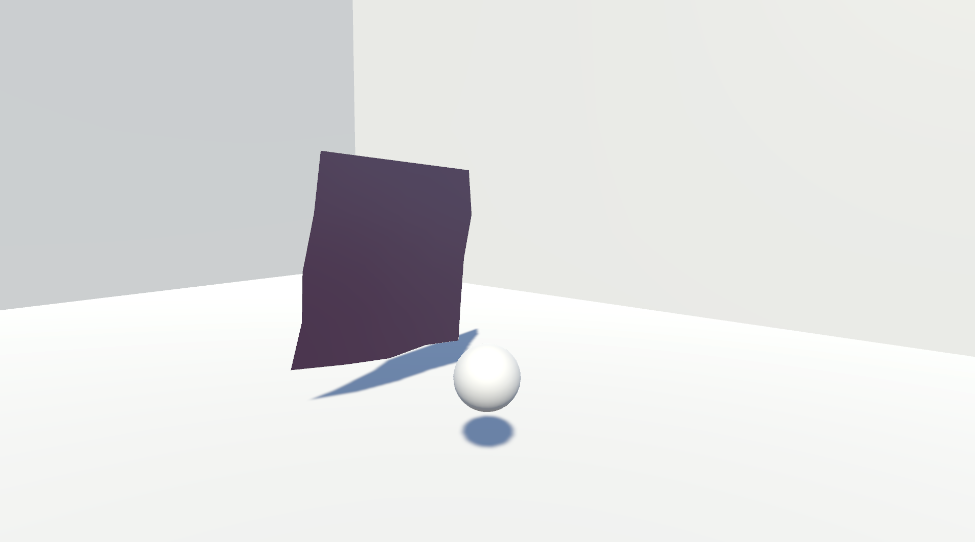
\includegraphics[width=0.8\textwidth]{Imagenes/Exp/Recurrencia/RNN.png}
        \caption{Tela simulada a través de RNN.}
        \label{fig:rnnexp}
    \end{minipage}
    \hfill
    \begin{minipage}{0.48\textwidth}
        \centering
        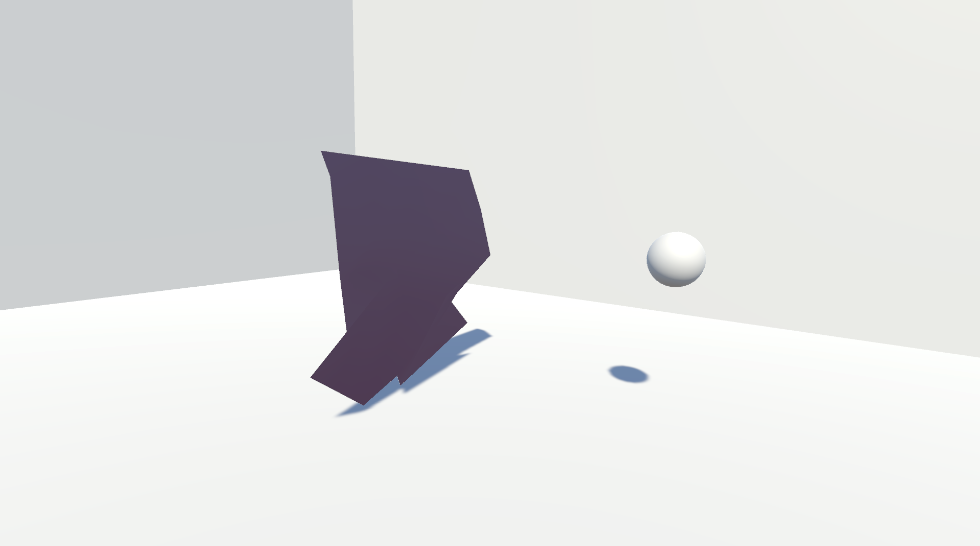
\includegraphics[width=0.8\textwidth]{Imagenes/Exp/Recurrencia/MLP.png}
        \caption{Tela simulada a través de MLP.}
        \label{fig:mlpexp}
    \end{minipage}
\end{figure}

Se concluyen las siguientes puntuaciones de calidad visual: 
\begin{table}[H]
    \begin{center}
        \begin{tabular}{ | m{2cm} |  m{2.6cm} | m{2.8cm} | m{2.6cm} | m{2.7cm} |}
        \hline \textbf{Prueba} & \textbf{Reactividad} & \textbf{Conservación} & \textbf{Estabilidad} & \textbf{Credibilidad} \\ \hline
            MLP & 1/3 & 0/3 & 1/3 & 2/3  \\ \hline
            RNN & 1/3 & 3/3 & 3/3 & 2/3 \\ \hline
        \end{tabular}
    \end{center}
    \caption{Resultados del entrenamiento en base a la percepción (Recurrencia).}
    \label{tab:visResultsRec}
\end{table}

Con esta metodología y técnicas concretas, compensa mantener la recurrencia para evitar la pérdida de estructura de la tela. No obstante, se planteará encontrar posteriormente una técnica más restrictiva en cuanto a estuctura que permita aprovechar los bajos tiempos de entrenamiento e inferencia del MLP.

\section{Unrolling}
Como se ha expuesto anteriormente, esta es una técnica que resulta ser muy útil en la autocorreción del modelo; este experimento pretende valorar su repercusión en la calidad visual de la simulación. Se realiza el experimento modificando la secuencia de entrada del RNN entre 1 y 24 frames futuras, de tal modo, pueden compararse los efectos del unrolling con un modelo análogo que solo infiere un frame, es decir, un modelo sin unrolling. El resto de parámetros se mantienen consistentes con los de la prueba anterior. \newline

En la siguiente tabla, \ref{tab:rendResultsUnroll}, pueden verse los resultados en cuanto al rendimiento. Es interesante subrayar la diferencia entre los errores medios por vértice, esto se debe a que dada la tendencia del modelo con unrolling a la autocorrección la inferencia de cada paso puede ser menos acertada, aunque a largo plazo eso le permite corromperse menos.

\begin{table}[H]
    \begin{center}
        \begin{tabular}{ | m{2.2cm} |  m{2.8cm} | m{2.8cm} | m{2.6cm} | m{1.2cm} |}
        \hline \textbf{Rolling steps} & \textbf{T entrenamiento} & \textbf{T inferencia} & \textbf{Error medio por vértice} & \textbf{FPS} \\ \hline
            1 & 1.5h(gpu) & 2.17ms & 0.0008m & 427 \\ \hline
            24 & 18h(gpu) & 2.17ms & 0.0013m & 429 \\ \hline
        \end{tabular}
    \end{center}
    \caption{Resultados de los entrenamientos en base al rendimiento (Unrolling).}
    \label{tab:rendResultsUnroll}
\end{table}

Contemplando ambas simulaciones en ejecución, es clara la diferencia en la conservación de la estructura de la geometría. Si bien, al contar con el resto de técnicas implementadas, la corrupción de la forma de la tela no es tan exagerada. Estos resultados visuales pueden compararse en la figura \ref{fig:estrucUnfold}. 

\begin{figure}[H]
    \centering
    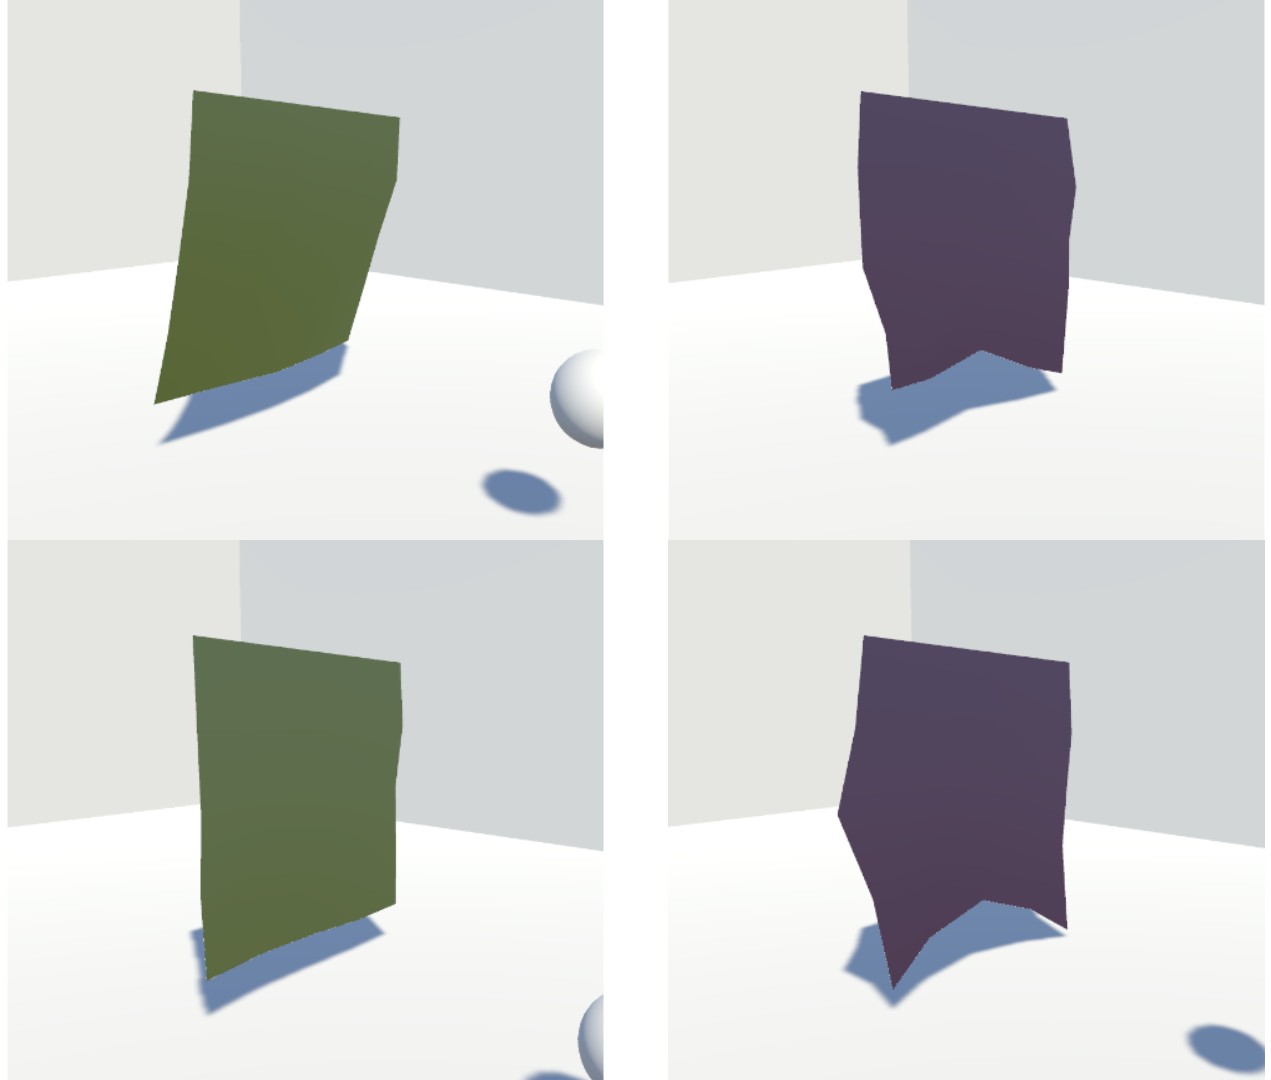
\includegraphics[width=0.7\textwidth]{Imagenes/estructuraUnfolding.png}
    \caption{Estado de la geometría trás 100 segundos de ejecución. En la izquierda, en verde, la tela entrenada con 24 frames de unrolling y en la derecha, en morado, la entrenada sin emplear esta técnica.}
    \label{fig:estrucUnfold}
\end{figure}

Por otro lado, es interesante recalcar que el modelo sin unrolling permite más reactividad a la tela. Al contrario, utilizando la técnica, la inferencia tiene en cuenta el cambio de velocidad y aceleración provocados, por lo que las predicciones tienden a ser más cautelosas y se reduce el movimiento total.

\begin{table}[H]
    \begin{center}
        \begin{tabular}{ | m{2cm} |  m{2.6cm} | m{2.8cm} | m{2.6cm} | m{2.7cm} |}
        \hline \textbf{Rolling steps} & \textbf{Reactividad} & \textbf{Conservación} & \textbf{Estabilidad} & \textbf{Credibilidad} \\ \hline
            1 & 2/3 & 1/3 & 3/3 & 2/3 \\ \hline
            24 & 1/3 & 3/3 & 3/3 & 2/3 \\ \hline
        \end{tabular}
    \end{center}
    \caption{Resultados de los entrenamientos en base a la percepción (Unrolling).}
    \label{tab:visResultsUnfold}
\end{table}

\section{Velocidad}
Al utilizar secuencias de frames para el entrenamiento, teniendo las posiciones de cada vértice, la velocidad puede ser inferida. Sin embargo, la secuencia de las velocidades aporta al modelo una conciencia acerca de la aceleración y deceleración de los vértices, por lo que se considera importante medir el impacto en este experimento. En el momento de medir los parámetros mediante el random forest en el apartado \ref{sec:Dataset} se resalta la velocidad en el eje X como la información de la simulación más relevante, y podría resultar la información clave para aprender a gestionar la inercia.

No obstante, de forma previa al experimento se pueden intuir dos implicaciones arriesgadas de emplear la velocidad como parámetro. En primer lugar, para generar el tensor de entrada es necesario calcular primero la velocidad de cada punto de la tela en cada frame, lo cual supone un aumento en el coste computacional en la simulación. Pero sobre todo, la velocidad otorga una mayor sensibilidad al error en el modelo, por lo que se puede intuir que sufrirá una mayor cantidad de desplazamientos erráticos.

Se quiere comprobar si la información que aporta la velocidad compensa los márgenes de error elevados.
Ambas pruebas siguen los parámetros:
\begin{table}[H]
    \begin{center}
        \begin{tabular}{ | m{2.2cm} | m{2cm} | m{1.2cm} | m{2.1cm} | m{2.4cm} | m{2.2cm} | }
        \hline \textbf{Windows size} & \textbf{Rollout steps} & \textbf{Noise} & \textbf{Learning rate} & \textbf{Tamaño dataset} & \textbf{Batch size} \\ \hline
            16 & 24 & 3\% & 0.001 & 25000 & 32 \\ \hline
        \end{tabular}
            \end{center}
    \caption{Hiperparámetros y configuración del entrenamiento (Velocidad).}
    \label{tab:randomTrainingVel}
\end{table}

El cálculo del loss y unrolling en ambos pruebas es equivalente, únicamente difieren por el nuevo parámetro recibido, la velocidad de cada vértice de la tela. 
Los resultados son los siguientes:
\begin{table}[H]
    \begin{center}
        \begin{tabular}{ | m{2.2cm} |  m{2.8cm} | m{2.8cm} | m{2.6cm} | m{1.2cm} |}
        \hline \textbf{Prueba} & \textbf{T entrenamiento} & \textbf{T inferencia} & \textbf{Error medio por vértice} & \textbf{FPS} \\ \hline
            Pos & 18h(gpu) & 2.25ms & 0.0013m & 413 \\ \hline
            Pos + Vel & 18h(gpu) & 2.26.0ms & 0.0009m & 411 \\ \hline
        \end{tabular}
    \end{center}
    \caption{Resultados del entrenamiento en base al rendimiento (Velocidad).}
    \label{tab:rendResultsVel}
\end{table}

En este experimento, podemos observar que el error de vértice observado en el entrenamiento y testing con la velocidad como parámetro es bastante inferior. El tiempo de entrenamiento prácticamente no sube, ambos rozan las 18h (a causa de la técnica de unrolling). Las FPS y tiempo de inferencia caen ligeramente al contar con tres parámetros más de entrada (vx, vy, vz).

Pese a que el error de vértice de la prueba con velocidad parece bajo, esto no se trasmite en la simulación final. La simulación muestra reacción adecuada, pero coge inercia con mucha más rapidez, y realiza movimientos exagerados. Esto perjudica la simulación, y provoca que la tela pierda la estructura a medida que avanza. En la figura \ref{fig:vel1} podemos apreciar como reacciona a tiempo a la colisión, pero realiza un movimiento más grande de lo necesario para dejar la bola pasar. En la siguiente imagen \ref{fig:vel2} se aprecia como ha quedado deformada la tela por este movimiento y posteriores. Aunque la tela se mantiene estable y no se dispara al infinito, las deformaciones se acumulan y deforman la tela permanentemente a medida que avanza el tiempo. Adicionalmente, es interesante mencionar como varía mucho más la velocidad (de forma no natural) a la que reacciona y vuelve al reposo la tela en comparación con la RNN basada en posiciones.

\begin{figure}[H]
    \begin{minipage}{0.48\textwidth}
        \centering
        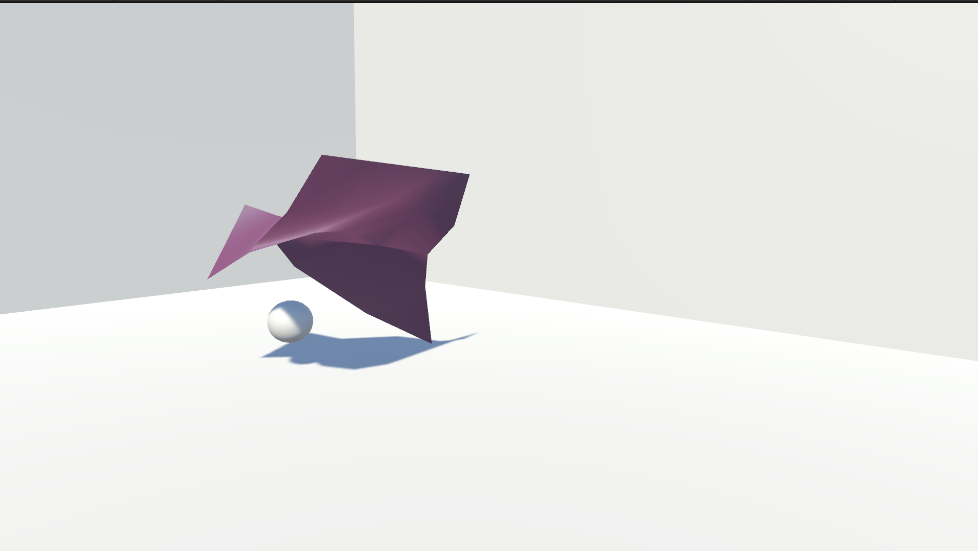
\includegraphics[width=0.8\textwidth]{Imagenes/Exp/Velocidad/MovimientoExagerado.png}
        \caption{Movimientos exagerados al comienzo de la simulación con velocidad.}
        \label{fig:vel1}
    \end{minipage}
    \hfill
    \begin{minipage}{0.48\textwidth}
        \centering
        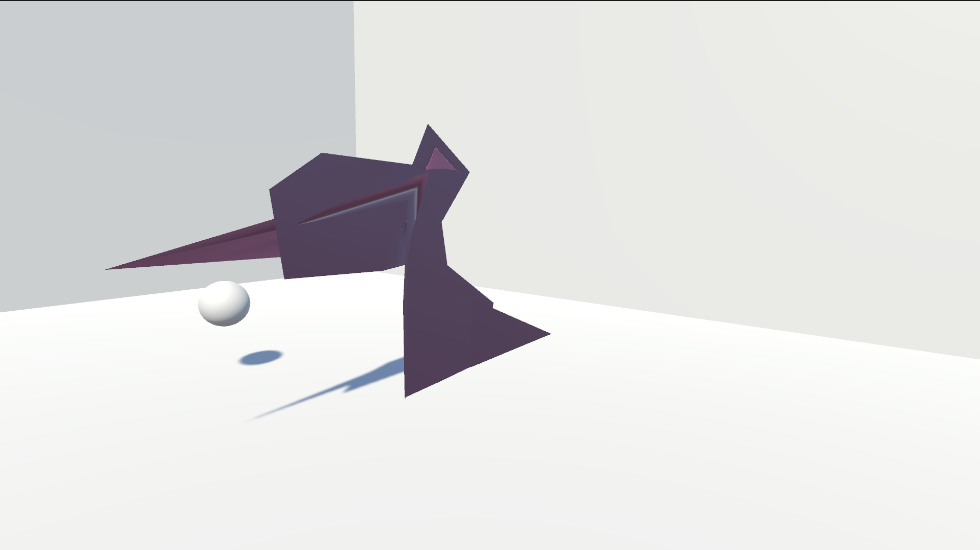
\includegraphics[width=0.8\textwidth]{Imagenes/Exp/Velocidad/Deformado.png}
        \caption{Ejemplo de deformación de la tela pasado un minuto en la simulación con velocidad.}
        \label{fig:vel2}
    \end{minipage}
\end{figure}

Visto esto, se concluyen las siguientes puntuaciones a nivel visual:
\begin{table}[H]
    \begin{center}
        \begin{tabular}{ | m{2.2cm} |  m{2.8cm} | m{2.8cm} | m{2.8cm} | m{2.8cm} |}
        \hline \textbf{Prueba} & \textbf{Reactividad} & \textbf{Conservación} & \textbf{Estabilidad} & \textbf{Credibilidad} \\ \hline
            Pos         & 1/3 & 3/3 & 3/3 & 2/3 \\ \hline
            Pos + Vel   & 2/3 & 0/3 & 1/3 & 1/3 \\ \hline
        \end{tabular}
    \end{center}
    \caption{Resultados del entrenamiento en base a la percepción (Velocidad).}
    \label{tab:visResults}
\end{table}

Se concluye que con este contexto, emplear la velocidad como parámetro no produce mejoras frente a usar únicamente las posiciones y sdfs. Los movimientos exagerados y un tanto erráticos perjudican notablemente la naturalidad de la tela.
\section{PCA}
Resulta interesante introducir un modelo que se valga de un PCA para reducir la dimensión de los parámetros de entrada, que ayude a optimizar y facilite el escalado a mallas de gran tamaño. Esta técnica permanece como una de las más utilizadas para alcanzar mejoras de rendimiento. En este experimento, utilizando el método del umbral de varianza, se calcula el mínimo de características necesarias para alcanzar un gran porcentaje de la variabilidad de los datos con un umbral de varianza del 95\%, reduciendo drásticamente el número de componentes. 

Se aplica el PCA sobre la misma versión de RNN que incorpora unrolling empleada en los experimentos anteriores. Esta combinación resulta similar a lo propuesto por \cite{holden_subspace_2019}, a excepción de la incorporación de la recurrencia como método de contención de la inercia de la simulación. Como se explica anteriormente en la descripción del PCA \ref{alg:pca}, la diferencia de ambos elementos reside en que el modelo opera sobre deltas de posiciones o deltas de las posiciones en el subespacio.

Ambas pruebas comparten los parámetros:
\begin{table}[H]
    \begin{center}
        \begin{tabular}{ | m{2.2cm} | m{2cm} | m{1.2cm} | m{2.1cm} | m{2.4cm} | m{2.2cm} | }
        \hline \textbf{Windows size} & \textbf{Rollout steps} & \textbf{Noise} & \textbf{Learning rate} & \textbf{Tamaño dataset} & \textbf{Batch size} \\ \hline
            16 & 24 & 3\% & 0.001 & 25000 & 32 \\ \hline
        \end{tabular}
            \end{center}
    \caption{Hiperparámetros y configuración del entrenamiento (PCA).}
    \label{tab:randomTrainingPCA}
\end{table}

Los resultados son los siguientes:
\begin{table}[H]
    \begin{center}
        \begin{tabular}{ | m{2.2cm} |  m{2.8cm} | m{2.8cm} | m{2.6cm} | m{1.2cm} |}
        \hline \textbf{Prueba} & \textbf{T entrenamiento} & \textbf{T inferencia} & \textbf{Error medio por vértice} & \textbf{FPS} \\ \hline
            RNN & 18h(gpu) & 2.17ms & 0.0013m & 444 \\ \hline
            RNN + PCA & 19h(gpu) & 1.89ms & 0.005298m & 472 \\ \hline
        \end{tabular}
    \end{center}
    \caption{Resultados del entrenamiento en base al rendimiento (PCA).}
    \label{tab:rendResultsPCA}
\end{table}

El entrenamiento que incorpora PCA tarda un poco más que el básico, pero este coste de entrenamiento se puede decrementar fácilmente si se realiza el cómputo de frames PCA a la hora de guardar el dataset para reducirlo. El PCA aporta al modelo una inferencia más rápida y aporta un incremento de tasa de frames de un 6,3\%. Como era de esperar, al reducir los datos, el error de vértice aumenta notablemente.

La mejor característica que aporta el PCA sobre el RNN básico es la capacidad total de mantener la estructura de la tela a largo plazo. Es elástica, cuando el colisionador está suficientemente alejado sabe volver a la posición de reposo de forma natural, y no padece deformaciones permanentes. No obstante, la actitud que adopta en las colisiones y los momentos inmediatos a ellas es errática. Se observa temblor en los movimientos, elección errónea de la dirección al choque y adopción de poses encogidas para dejar pasar el colisionador. De forma similar a lo visto en el experimento de la velocidad, esta tela con PCA adopta velocidades aleatorias, particularmente durante el cambio de colisionar y volver su fase de reposo (en la que en el dataset original siempre mantiene inercia y no llega a parar del todo). En la siguiente figura se puede apreciar como la tela se comprime hacia un lado para dejar pasar el colisionador (que avanza desde el fondo de la escena), y se recupera sin problema más tarde.
\begin{figure}[H]
    \begin{minipage}{0.48\textwidth}
        \centering
        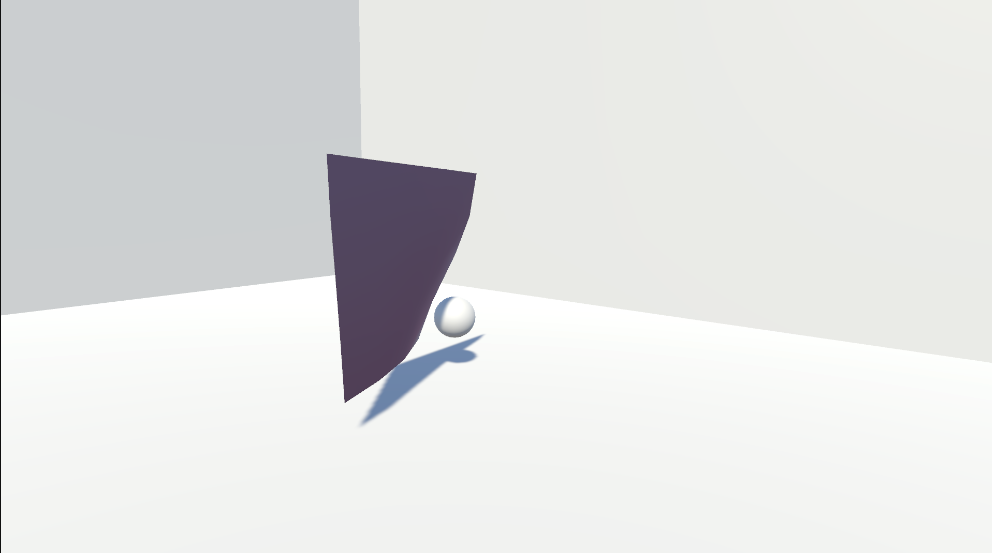
\includegraphics[width=0.8\textwidth]{Imagenes/Exp/PCA/Paso.png}
        \caption{La tela con PCA se hace a un lado para dejar pasar al colisionador, que viene del fondo.}
        \label{fig:pca1}
    \end{minipage}
    \hfill
    \begin{minipage}{0.48\textwidth}
        \centering
        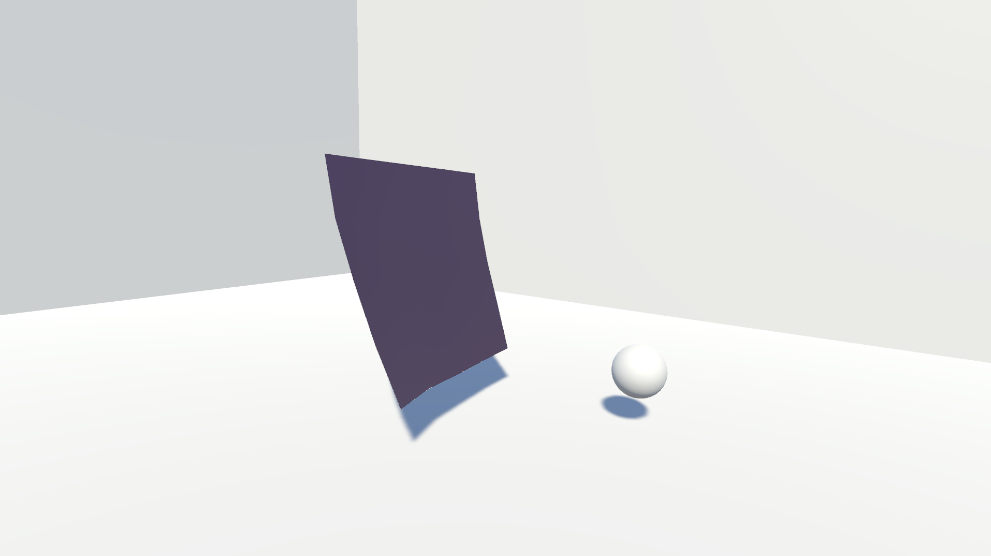
\includegraphics[width=0.8\textwidth]{Imagenes/Exp/PCA/Reposo.png}
        \caption{Tras lo ocurrido en \ref{fig:pca1}, la tela con PCA recupera su estructura de reposo y su movimiento con inercia entre colisiones.}
        \label{fig:pca2}
    \end{minipage}
\end{figure}
Adicionalmente a este experimento, se han realizado pequeñas pruebas que han confirmado que la gestión de colisiones mejora notablemente con el aumento de tamaño del dataset, como es de esperar. Se califican los resultados obtenidos de la siguiente forma:
\begin{table}[H]
    \begin{center}
        \begin{tabular}{ | m{2.2cm} |  m{2.8cm} | m{2.8cm} | m{2.8cm} | m{2.8cm} |}
        \hline \textbf{Prueba} & \textbf{Reactividad} & \textbf{Conservación} & \textbf{Estabilidad} & \textbf{Credibilidad} \\ \hline
            RNN         & 1/3 & 3/3 & 3/3 & 2/3 \\ \hline
            RNN + PCA & 1/3 & 2/3 & 3/3 & 1/3 \\ \hline
        \end{tabular}
    \end{center}
    \caption{Resultados del entrenamiento en base a la percepción (PCA).}
    \label{tab:visResultsPCA}
\end{table}

En conclusión, se observa una mejora de rendimiento en la versión que incopora PCA, aunque esta también presenta un mayor error de vértice y movimientos aleatorios. La estabilidad y buena recuperación a la pose de reposo son destacables, y merecen más investigación al respecto, pero las colisiones como tal hacen que no sea una tela creíble y natural usable. 

\section{Aplicación para la visualización de los experimentos}
\label{sec:App}

Para poder visualizar los resultados, se ha implementado una aplicación disponible en el repositorio del proyecto. La interfaz permite acceder a los distintos experimentos llevados a cabo a través de un menú principal, que puede verse en la figura \ref{fig:appA}. 
\begin{figure}[H]
    \centering
    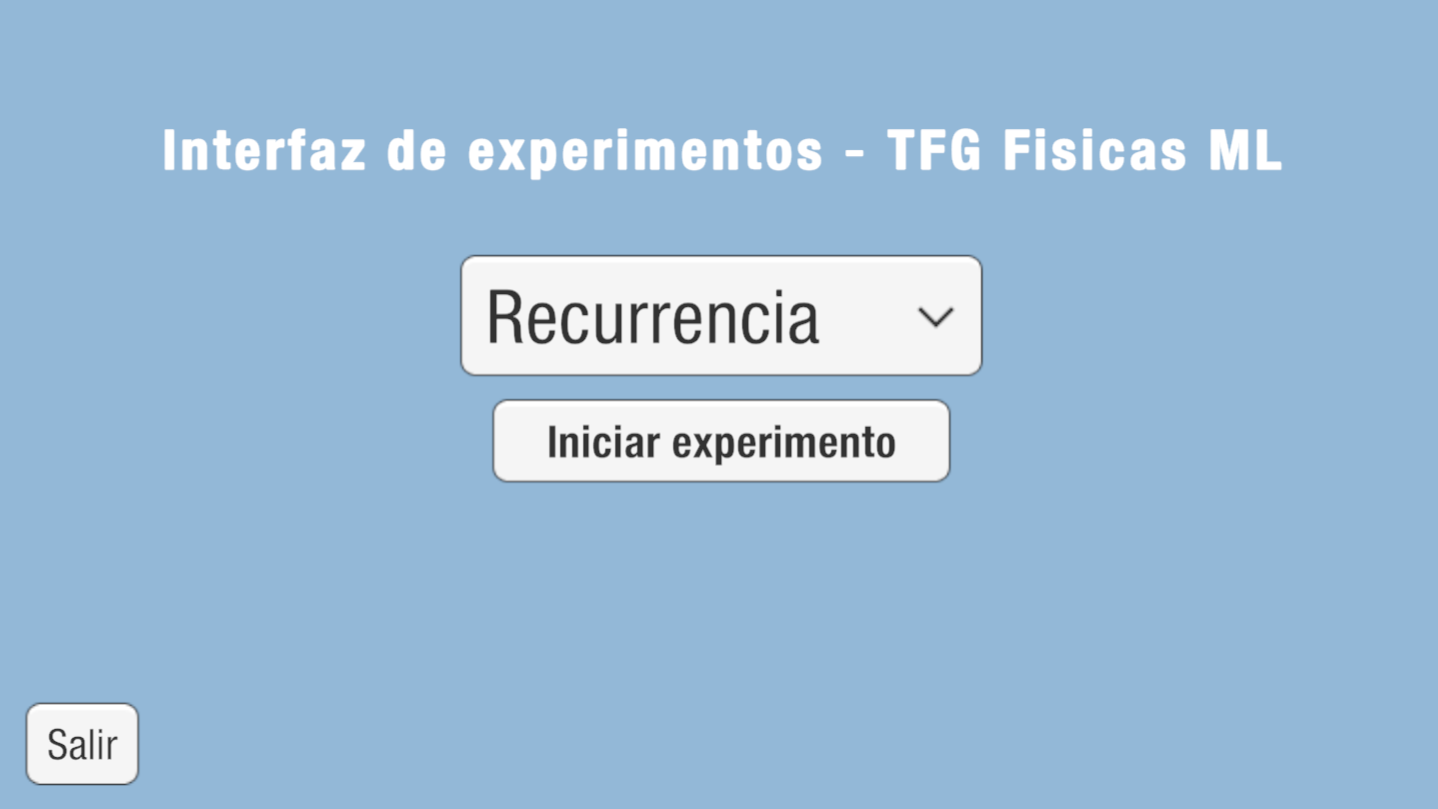
\includegraphics[width=0.7\textwidth]{Imagenes/AplicacionA.png}
    \caption{Menú principal de la aplicación.}
    \label{fig:appA}
\end{figure}

En cada experimento pueden activarse distintas versiones de los modelos entrenados, así como la simulación de cloth de Unity. Además de la comparación visual que esto permite, se generan diferentes métricas del rendimiento en tiempo de ejecución de cada simulación: La media de frames por segundo y la máxima y mínima tasas alcanzadas en el tiempo especificado. Las ejecuciones pueden pararse en cualquier momento con el botón de ``Stop'', pero se recomienda mantener cada simulación en curso durante al menos un minuto para obtener métricas más veraces.
\begin{figure}[H]
    \centering
    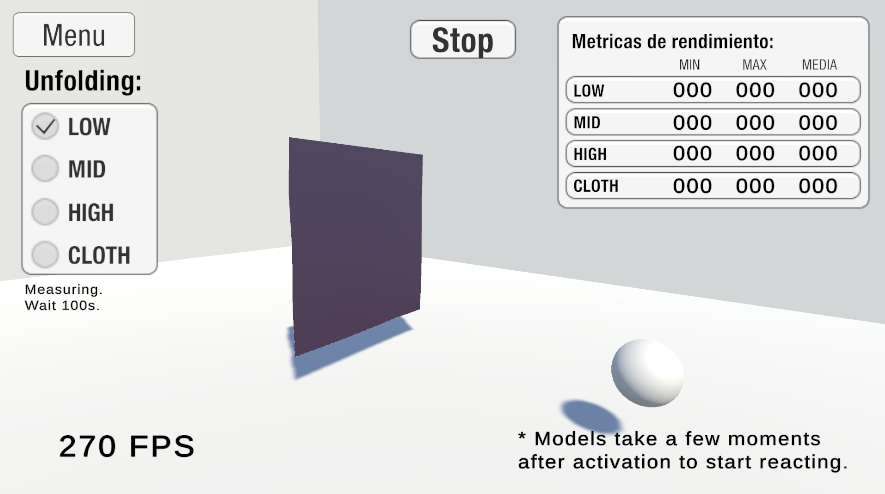
\includegraphics[width=0.7\textwidth]{Imagenes/AplicacionB.png}
    \caption{Ejemplo de la ejecución de una simulación de un experimento.}
    \label{fig:appB}
\end{figure}